\twocolumn[\colorsection{Potencial eléctrico}]
\setcounter{figure}{0}
%
\begin{Exercise}
  ¿Cuál es la energía necesaria para ubicar cuatro cargas de $\SI{3.0}{\micro\coulomb}$ en las esquinas de un cuadrado cuyos lados miden $\SI{7.5}{\centi\metre}$?
\end{Exercise}
\begin{Answer}
  $\SI{5.85}{\joule}$
\end{Answer}
%
\begin{Exercise}
  Una carga puntual de $\SI{4.0}{\nano\coulomb}$ está situada en el origen, y otra carga puntual de $\SI{-3.0}{\nano\coulomb}$ está sobre el eje $x$ en la posición $x = \SI{0.20}{\metre}$. ¿Dónde debe situarse sobre el eje $x$, una tercera carga de $\SI{2.0}{\nano\coulomb}$, para que la energía potencial del sistema formado por las tres cargas sea igual a cero?
\end{Exercise}
\begin{Answer}
	\begin{minipage}[t]{.4\textwidth}
    $x = \SI{-0.10}{\metre}$ o $x = \SI{0.074}{\metre}$
  \end{minipage}
\end{Answer}
%
\begin{Exercise}
  Una carga puntual $q_1 = \SI{2.40}{\nano\coulomb}$ se mantiene estacionaria en el origen. Una segunda carga puntual $q_2 = \SI{-4.30}{\nano\coulomb}$ se desplaza desde la posición $\va*{r}_0 =\SI{0.150}{\metre}\vu{x} + \SI{0}{\metre}\vu{y}$ hasta la posición $\va*{r}_f =\SI{0.250}{\metre}\vu{x} + \SI{0.250}{\metre}\vu{y}$. ¿Cuánto varió la energía potencial de la carga $q_2$?
\end{Exercise}
\begin{Answer}
  $\SI{3.57E-7}{\joule}$
\end{Answer}
%
\begin{Exercise}
  Un pequeño objeto tiene una carga neta $q_1 = \SI{2.80}{\micro\coulomb}$ y se mantiene en una posición fija por medio de soportes aislantes. Un segundo objeto pequeño, con carga neta $q_2 = \SI{7.80}{\micro\coulomb}$ y una masa de $\SI{1.50}{\gram}$, es proyectado hacia $q_1$. Cuando los dos objetos están a una distancia de $\SI{0.800}{\metre}$ uno de otro, $q_2$ se mueve hacia $q_1$ con una rapidez de $\SI{22.0}{\metre/\second}$. Suponga que los objetos pueden considerarse como cargas puntuales, ¿qué tan cerca de $q_1$ llega $q_2$?
\end{Exercise}
\begin{Answer}
  $\SI{0.323}{\metre}$
\end{Answer}
%
\begin{Exercise}
  \textbf{electronvolt:} Un electronvolt ($\SI{1}{eV}$) es una unidad de energía que equivale a la variación de energía potencial de un electrón que se desplaza a través de una diferencia de potencial de $\SI{1}{\volt}$. \textit{a}) Verifique la siguiente equivalencia: \[\SI{1}{eV} = \SI{1.602E-19}{\joule}~.\] \textit{b}) Calcule la energía (en eV y en J) de un electrón que ha sido acelerado desde el reposo, a través de una diferencia de potencial de $\SI{100}{\volt}$. \textit{c}) Calcule la velocidad que alcanza ese electrón.
\end{Exercise}
\begin{Answer}
	\begin{minipage}[t]{.4\textwidth}
    \textit{b}) $\SI{100}{eV} = \SI{1.602E-17}{\joule}$\\ \textit{c}) $\SI{5.93E6}{\metre/\second}$
  \end{minipage}
\end{Answer}
%
\begin{Exercise}
  Calcule el potencial eléctrico en el centro de un cuadrado de $\SI{1}{\metre}$ de lado, si en sus vértices se ubican las siguientes cargas: $q_1 = \SI{10}{\nano\coulomb}$; $q_2 = \SI{-20}{\nano\coulomb}$; $q_3 = \SI{30}{\nano\coulomb}$ y $q_4 = \SI{20}{\nano\coulomb}$.
\end{Exercise}
\begin{Answer}
  $\SI{509}{\volt}$
\end{Answer}
%
\begin{Exercise}\label{p:potencial01}
  Para la distribución de cargas mostrada en la figura \ref{f:potencial01}, donde $q_1 = \SI{3.1}{\micro\coulomb}$ y $q_2 = \SI{2.4}{\micro\coulomb}$ están sobre el plano $xy$, calcule: \textit{a}) el potencial eléctrico en el origen de coordenadas, \textit{b}) el potencial eléctrico en la posición $\va*{r} =\SI{0.25}{\metre}\vu{z}$.
\end{Exercise}
\begin{Answer}
	\begin{minipage}[t]{.4\textwidth}
    \textit{a}) $\SI{1.98E5}{\volt}$\\ \textit{b}) $\SI{1.4E5}{\volt}$
  \end{minipage}
\end{Answer}
%
\begin{center}
  \begin{tikzpicture}[scale=0.5]
    %Axis
    \draw[axis] (-1,0) -- (5,0) node [below, pos=1.1] {$x$};
    \draw[axis] (0,-1) -- (0,5) node [left, pos=1.05] {$y$};
    \fill [black](2.5,0) circle(5pt) node[above] {$q_1$} node[below] {$0.25\text{ m}$};
    \fill [black](0,2.5) circle(5pt) node[right] {$q_2$} node[left] {$0.25\text{ m}$};
  \end{tikzpicture}
  \captionof{figure}{Problema \ref{p:potencial01}\label{f:potencial01}}
\end{center}
%
\begin{Exercise}\label{p:potencial02}
  Un dipolo de cargas $\pm q$ y separación $d$ ($p=qd$) está colocado sobre el eje $\vu{i}$ como se muestra en la figura \ref{f:potencial02}. \textit{a}) Verifique que el potencial en el punto $P$ es:
  \begin{flalign*}
    V_P &= \dfrac{1}{4\pi\varepsilon_o} \dfrac{p}{x^2-\dfrac{d^2}{4}}
  \end{flalign*}
  \textit{b}) A partir de la expresión del ítem \textit{a}, verifique que el trabajo necesario para transportar una carga $Q$ muy distante hasta un punto situado sobre el eje $\vu{i}$, a una distancia $a$ del centro del dipolo es:
  \begin{flalign*}
    W = QV_a &= \dfrac{Q}{4\pi\varepsilon_o} \dfrac{p}{a^2-\dfrac{d^2}{4}}
  \end{flalign*}
  \textit{c}) Verifique que el potencial en $P$ cuando $x \gg d$ puede ser aproximado por:
  \begin{flalign*}
    V_P &= \dfrac{1}{4\pi\varepsilon_o} \dfrac{p}{x^2}
  \end{flalign*}
  \textit{d}) A partir del resultado anterior y usando $\va*{E} = -\nabla V$, obtenga la siguiente expresión para el campo eléctrico en el punto $P$ cuando $x \gg d$:
  \begin{flalign*}
    \va*{E}_P &= \dfrac{1}{2\pi\varepsilon_o} \dfrac{p}{x^3}\vu{i}
  \end{flalign*}
\end{Exercise}
%
\begin{center}
  \begin{tikzpicture}[scale=0.5]
    %Axis
    \draw[axis] (-5,0) -- (7 ,0) node [below, pos=1] {$i$};
    \draw[axis] (0,-0.5) -- (0,2) node [left, pos=1] {$j$};
    \fill [black](-2.5,0) circle(5pt) node[above] {$-q$};
    \fill [black](2.5,0) circle(5pt) node[above] {$q$};
    \fill [red](4.5,0) circle(5pt) node[above] {$P$};
    \draw [{latex}-{latex}] (0,-1) -- (4.5, -1) node [midway, below] {$x$};
  \end{tikzpicture}
  \captionof{figure}{Problema \ref{p:potencial02}\label{f:potencial02}}
\end{center}
%
% Agregar lo siguiente en las opciones de axis del objeto tikzpicture:
% width=0.85\textwidth, height=\axisdefaultheight,
\begin {figure*}%[!hbtp]
  \centering
  \begin{adjustbox}{width=\textwidth}
    % This file was created with tikzplotlib v0.10.1.
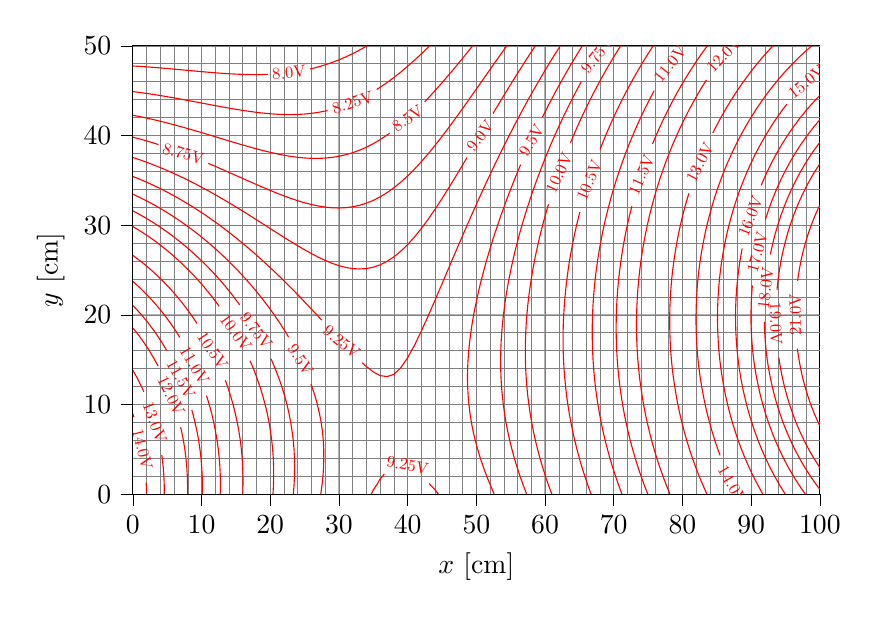
\begin{tikzpicture}

\definecolor{darkgray176}{RGB}{176,176,176}
\definecolor{gray}{RGB}{128,128,128}

\begin{axis}[width=0.85\textwidth,
  height=\axisdefaultheight,
tick align=outside,
tick pos=left,
x grid style={darkgray176},
xlabel={\(\displaystyle x\) [cm]},
xmajorgrids,
xmin=0, xmax=100,
xtick style={color=black},
y grid style={darkgray176},
ylabel={\(\displaystyle y\) [cm]},
ymajorgrids,
ymin=0, ymax=50,
ytick style={color=black}
]
\addplot [very thin, gray]
table {%
0 2
100 2
};
\addplot [very thin, gray]
table {%
0 4
100 4
};
\addplot [very thin, gray]
table {%
0 6
100 6
};
\addplot [very thin, gray]
table {%
0 8
100 8
};
\addplot [very thin, gray]
table {%
0 10
100 10
};
\addplot [very thin, gray]
table {%
0 12
100 12
};
\addplot [very thin, gray]
table {%
0 14
100 14
};
\addplot [very thin, gray]
table {%
0 16
100 16
};
\addplot [very thin, gray]
table {%
0 18
100 18
};
\addplot [very thin, gray]
table {%
0 20
100 20
};
\addplot [very thin, gray]
table {%
0 22
100 22
};
\addplot [very thin, gray]
table {%
0 24
100 24
};
\addplot [very thin, gray]
table {%
0 26
100 26
};
\addplot [very thin, gray]
table {%
0 28
100 28
};
\addplot [very thin, gray]
table {%
0 30
100 30
};
\addplot [very thin, gray]
table {%
0 32
100 32
};
\addplot [very thin, gray]
table {%
0 34
100 34
};
\addplot [very thin, gray]
table {%
0 36
100 36
};
\addplot [very thin, gray]
table {%
0 38
100 38
};
\addplot [very thin, gray]
table {%
0 40
100 40
};
\addplot [very thin, gray]
table {%
0 42
100 42
};
\addplot [very thin, gray]
table {%
0 44
100 44
};
\addplot [very thin, gray]
table {%
0 46
100 46
};
\addplot [very thin, gray]
table {%
0 48
100 48
};
\addplot [very thin, gray]
table {%
0 50
100 50
};
\addplot [very thin, gray]
table {%
2 0
2 50
};
\addplot [very thin, gray]
table {%
4 0
4 50
};
\addplot [very thin, gray]
table {%
6 0
6 50
};
\addplot [very thin, gray]
table {%
8 0
8 50
};
\addplot [very thin, gray]
table {%
10 0
10 50
};
\addplot [very thin, gray]
table {%
12 0
12 50
};
\addplot [very thin, gray]
table {%
14 0
14 50
};
\addplot [very thin, gray]
table {%
16 0
16 50
};
\addplot [very thin, gray]
table {%
18 0
18 50
};
\addplot [very thin, gray]
table {%
20 0
20 50
};
\addplot [very thin, gray]
table {%
22 0
22 50
};
\addplot [very thin, gray]
table {%
24 0
24 50
};
\addplot [very thin, gray]
table {%
26 0
26 50
};
\addplot [very thin, gray]
table {%
28 0
28 50
};
\addplot [very thin, gray]
table {%
30 0
30 50
};
\addplot [very thin, gray]
table {%
32 0
32 50
};
\addplot [very thin, gray]
table {%
34 0
34 50
};
\addplot [very thin, gray]
table {%
36 0
36 50
};
\addplot [very thin, gray]
table {%
38 0
38 50
};
\addplot [very thin, gray]
table {%
40 0
40 50
};
\addplot [very thin, gray]
table {%
42 0
42 50
};
\addplot [very thin, gray]
table {%
44 0
44 50
};
\addplot [very thin, gray]
table {%
46 0
46 50
};
\addplot [very thin, gray]
table {%
48 0
48 50
};
\addplot [very thin, gray]
table {%
50 0
50 50
};
\addplot [very thin, gray]
table {%
52 0
52 50
};
\addplot [very thin, gray]
table {%
54 0
54 50
};
\addplot [very thin, gray]
table {%
56 0
56 50
};
\addplot [very thin, gray]
table {%
58 0
58 50
};
\addplot [very thin, gray]
table {%
60 0
60 50
};
\addplot [very thin, gray]
table {%
62 0
62 50
};
\addplot [very thin, gray]
table {%
64 0
64 50
};
\addplot [very thin, gray]
table {%
66 0
66 50
};
\addplot [very thin, gray]
table {%
68 0
68 50
};
\addplot [very thin, gray]
table {%
70 0
70 50
};
\addplot [very thin, gray]
table {%
72 0
72 50
};
\addplot [very thin, gray]
table {%
74 0
74 50
};
\addplot [very thin, gray]
table {%
76 0
76 50
};
\addplot [very thin, gray]
table {%
78 0
78 50
};
\addplot [very thin, gray]
table {%
80 0
80 50
};
\addplot [very thin, gray]
table {%
82 0
82 50
};
\addplot [very thin, gray]
table {%
84 0
84 50
};
\addplot [very thin, gray]
table {%
86 0
86 50
};
\addplot [very thin, gray]
table {%
88 0
88 50
};
\addplot [very thin, gray]
table {%
90 0
90 50
};
\addplot [very thin, gray]
table {%
92 0
92 50
};
\addplot [very thin, gray]
table {%
94 0
94 50
};
\addplot [very thin, gray]
table {%
96 0
96 50
};
\addplot [very thin, gray]
table {%
98 0
98 50
};
\addplot [very thin, gray]
table {%
100 0
100 50
};
\addplot [draw=none, draw=red]
table{%
x  y
34.0972176835943 50
34 49.9547442277928
33 49.5218841951851
32 49.124174138553
31.6598353571458 49
31 48.7607491086215
30 48.431890659444
29 48.1371976958045
28.4785070947643 48
28 47.8756440592398
27 47.6463987110537
26 47.4482580857582
25.7859525770838 47.4121832737974
};
\addplot [draw=none, draw=red]
table{%
x  y
19.6428603386127 46.8140411212797
19 46.7969734107752
18 46.7875707684262
17 46.7934646461131
16 46.8128420854785
15 46.8439382866875
14 46.8850456051439
13 46.9345209555475
12 46.9907916904096
11.8533223120803 47
11 47.0532254783566
10 47.1198821104574
9 47.1892670678344
8 47.2601037293291
7 47.3311911961116
6 47.4014033256896
5 47.4696869182144
4 47.5350591479725
3 47.5966043295983
2 47.653470104482
1 47.704863128318
0 47.7500443359339
};
\addplot [draw=none, draw=red]
table{%
x  y
43.202590672615 50
43 49.8436554684199
42 49.1054354292965
41.8502354414722 49
41 48.394908429438
40.4152797577244 48
40 47.7168823231278
39 47.07389565591
38.8776966742494 47
38 46.4665372928698
37.1757035517438 46
37 45.9001387667474
36 45.3736466221421
35.4951965813149 45.1300284910579
};
\addplot [draw=none, draw=red]
table{%
x  y
28.3409020573506 42.7864114460043
28 42.7236344114865
27 42.5775626458062
26 42.4672997678673
25 42.390471594098
24 42.3446289265954
23 42.3272758863281
22 42.3358962611148
21 42.3679776730272
20 42.4210334329571
19 42.4926220074304
18 42.5803640735636
17 42.6819571819221
16 42.7951880838555
15 42.9179428098177
14.3764326485329 43
14 43.0488317378326
13 43.1866934781329
12 43.3287989476831
11 43.4734812336496
10 43.6191869653374
9 43.7644761481606
8 43.9080207239663
7.35165738448983 44
7 44.0496436539146
6 44.1892993183441
5 44.3240762344326
4 44.4530147700322
3 44.5752423776178
2 44.689967621741
1 44.7964737340427
0 44.8941117811805
};
\addplot [draw=none, draw=red]
table{%
x  y
49.4660182550094 50
49 49.5514102829753
48.4093948150422 49
48 48.6091358414559
47.3399263897935 48
47 47.6794757881135
46.2516817392378 47
46 46.7667196407129
45.1374397094545 46
45 45.8754284814597
44 45.0102348822632
43.9875640727213 45
43 44.1738874658316
42.7803534034049 44
42.4755322633949 43.7550869288966
};
\addplot [draw=none, draw=red]
table{%
x  y
37.3763857285216 40.2591714509946
37 40.0475456421929
36.9064210214156 40
36 39.5381542082731
35 39.0885004695832
34.7758438845394 39
34 38.6942152574902
33 38.3579604481193
32 38.0788681665661
31.6528959824069 38
31 37.8529491424959
30 37.6791403587932
29 37.5552421062861
28 37.4779482861174
27 37.4438280844152
26 37.4493699473827
25 37.4910225718385
24 37.5652325822482
23 37.6684786724634
22 37.7973020873996
21 37.948333405352
20.7025132033866 38
20 38.1186752994622
19 38.3054543251907
18 38.505660548894
17 38.7165205707783
16 38.9354190521177
15.7188169665512 39
15 39.1615584912064
14 39.3922450087366
13 39.624791321661
12 39.8572541823167
11.3884354713452 40
11 40.0892745118728
10 40.3205047447659
9 40.5473425313434
8 40.7684425697176
7 40.982601529493
6.91787706310513 41
6 41.193112728575
5 41.3953979596127
4 41.5882008555989
3 41.7707516241719
2 41.9423802830539
1.64623179414111 42
1 42.105529120998
0 42.2583405720046
};
\addplot [draw=none, draw=red]
table{%
x  y
54.4242547265102 50
54 49.5365449026321
53.4976396860015 49
53 48.4525638881359
52.5780551461635 48
52 47.3615812573774
51.6632301068959 47
51 46.2670575019976
50.7506481681124 46
50 45.1729780803752
49.8374555587423 45
49 44.0838693689234
48.9203403308911 44
48 43.0048003432584
47.9953691631351 43
47.0547919724426 42
47 41.9401783412966
46.0960521974056 41
46 40.8975324969934
45.1123159075996 40
45 39.8836838896221
44.0944551010788 39
44 38.9057355198916
43.030350694403 38
43 37.9710561189413
42 37.0850832834074
41.8959746749483 37
41 36.2551364872811
40.6638442489904 36
40 35.4889159337649
39.2948119319828 35
39 34.7931087730703
38 34.1696710109549
37.6892237424879 34
37 33.6210206227518
36 33.1529139983366
35.6089725522436 33
35 32.7613776884851
34 32.4473399214186
33 32.2102248910559
32 32.0454461955464
31.539607350322 32
31 31.9471887556329
30 31.9118175192434
29 31.9347245360474
28.1407716825441 32
28 32.010212849478
27 32.1315135192712
26 32.2944540137256
25 32.4939481470506
24 32.7250450777505
23 32.9829640033404
22.94123129543 33
22 33.2620314579311
21 33.5596594911003
20 33.8719281720458
19.6124815419236 34
19 34.1953107350156
18 34.5269840767145
17 34.8637374139951
16.6067903747731 35
16 35.2039234702295
15 35.5451818075279
14 35.8843183593678
13.6627291000599 36
13 36.2216624652647
12 36.5547297876583
11 36.8804855416958
10.976082892204 36.8882354605896
};
\addplot [draw=none, draw=red]
table{%
x  y
3.72218615183459 38.9837995351492
3.65645049952239 39
3 39.1610874359127
2 39.3943121839007
1 39.6123377725597
0 39.8148070927148
};
\addplot [draw=none, draw=red]
table{%
x  y
58.590771634567 50
58 49.3091954442827
57.7309693211258 49
57 48.1304671677099
56.8881315797006 48
56.0588640236307 47
56 46.9265800551108
55.2393226351127 46
55 45.6977707982874
54.432689413281 45
54 44.4483126521239
53.6379572814491 44
53 43.181299091654
52.8540978739975 43
52.427859503101 42.4519210507183
};
\addplot [draw=none, draw=red]
table{%
x  y
48.6419454318295 37.5391160952692
48.2235522237014 37
48 36.7018427878865
47.4439083101288 36
47 35.4208604685773
46.6572104609507 35
46 34.1671445206395
45.8589471841604 34
45.0401674999665 33
45 32.949350714083
44.1865313086334 32
44 31.775784858552
43.2960839217891 31
43 30.664541829724
42.3528631632006 30
42 29.6282330759787
41.3324976629156 29
41 28.6795946088821
40.1955130095736 28
40 27.8312527302584
39 27.0914655330592
38.8524705856358 27
38 26.4630194516484
37.0732033084615 26
37 25.9629211465477
36 25.5746572902075
35 25.3094891744755
34 25.1574074513125
33 25.1083763140977
32 25.1524320554152
31 25.2797693250392
30 25.4808155379532
29 25.7462940440422
28.2165733557366 26
28 26.0655754839139
27 26.4249594563013
26 26.8235890692311
25.6006216689368 27
25 27.2495551593863
24 27.6980736714274
23.3652400892434 28
23 28.1642358722483
22 28.6413283822287
21.2722018193534 29
21 29.1274304792417
20 29.6167804075747
19.2280421786006 30
19 30.1080535282866
18 30.5972904387987
17.1765975103802 31
17 31.0828358586256
16 31.5627212135446
15.075348547518 32
15 32.0343422144243
14 32.4981078944075
13 32.949928388305
12.8898256065532 33
12 33.3922271104537
11 33.8205426738521
10.5747122094164 34
10 34.2364486217501
9 34.6386032091393
8.0629575269601 35
8 35.0238019350489
7 35.3979860849435
6 35.7538965101806
5.2770525499492 36
5 36.0931300803633
4 36.41925230554
3 36.7261538613894
2.04867472465353 37
2 37.0139418966283
1 37.2900330304474
0 37.546583457957
};
\addplot [draw=none, draw=red]
table{%
x  y
34.6985183906889 0
35 0.454511970748243
35.4727332686189 1
36 1.684260708172
36.3501986242067 2
36.6002700602266 2.25488800397992
};
\addplot [draw=none, draw=red]
table{%
x  y
43.1465974401465 1.18957858039395
43.3479834509281 1
44 0.466595361204628
44.480482518758 0
};
\addplot [draw=none, draw=red]
table{%
x  y
62.2146620876822 50
62 49.7383345134263
61.3866369467592 49
61 48.5163375424233
60.5810192908874 48
60 47.255384781746
59.7972275577003 47
59.0335141857365 46
59 45.9544880714147
58.2820912684611 45
58 44.6089410809879
57.5501961201927 44
57 43.2231423991827
56.8377453982917 43
56.1386738944684 42
56 41.7934035697468
55.4509806821259 41
55 40.3190510393265
54.781538613028 40
54.12472102342 39
54 38.8019925915709
53.4753609866877 38
53 37.2398683955973
52.8436947767182 37
52.2188641151429 36
52 35.6337637850644
51.6033065553271 35
51.0052218641332 34
51 33.9908723975933
50.4028575409938 33
50 32.2996379756111
49.8176127333096 32
49.2359153941171 31
49 30.5746957815169
48.6602475260086 30
48.0961113502171 29
48 28.8208415597003
47.526767411921 28
47 27.0418548226111
46.9750873478891 27
46.4100093226899 26
46 25.2377470487263
45.8599140615355 25
45.3016984536588 24
45 23.4294850181621
44.7474952381095 23
44.1913721773005 22
44 21.6338891842257
43.6243970017301 21
43.0642283366552 20
43 19.8764472484194
42.469514194828 19
42 18.1765914422151
41.8790836457383 18
41.2437240420722 17
41 16.5855927401143
40.5613357737909 16
40 15.194092631138
39.812553070794 15
39 14.0911495964876
38.8654851280019 14
38 13.3624855810527
37 13.1047187389705
36 13.2201526452497
35 13.6221452808772
34.4129903557396 14
34 14.215618317186
33.3724428206878 14.6578142323373
};
\addplot [draw=none, draw=red]
table{%
x  y
27.4867074417271 19.4078270727681
27 19.8093522143003
26.7844088827501 20
26 20.6295654735997
25.564889970407 21
25 21.439794419999
24.3152195365276 22
24 22.2374046698748
23.027949755615 23
23 23.0203090339624
22 23.7824561504022
21.7224647817479 24
21 24.5279022589584
20.3663535986986 25
20 25.2557602205186
19 25.9643746451519
18.9509758325057 26
18 26.6513341003808
17.4913675057687 27
17 27.3189633810134
16 27.9659035305182
15.9479798685514 28
15 28.5917448465523
14.3346964662296 29
14 29.1964727205632
13 29.7800266182723
12.6181213537458 30
12 30.3425708360569
11 30.8828427804425
10.7805506211606 31
10 31.403296834735
9 31.9003747875529
8.79599889022207 32
8 32.3784943800231
7 32.8331656243294
6.62124273691044 33
6 33.2680836061441
5 33.6814683688859
4.18543022638705 34
4 34.0714818438378
3 34.4447204359118
2 34.7933365507436
1.37088298413216 35
1 35.1211376954973
0 35.4311274868468
};
\addplot [draw=none, draw=red]
table{%
x  y
27.3514262379293 0
27.5361705766911 1
27.6727409441692 2
27.7606889776795 3
27.7989939626603 4
27.786015895724 5
27.7194348710733 6
27.5961739215361 7
27.4123015803044 8
27.1629092841479 9
27 9.51541193287876
26.8584755784236 10
26.5011483483749 11
26.0665996548619 12
26 12.1322397827294
25.9321187236478 12.2765655583552
};
\addplot [draw=none, draw=red]
table{%
x  y
22.6556277849322 17.5308849762878
22.2976997910263 18
22 18.3512605117774
21.4700891246201 19
21 19.5223669884757
20.5830332458368 20
20 20.6106657814771
19.6370946608561 21
19 21.6291605963731
18.6310466784557 22
18 22.5874954490221
17.5618781149036 23
17 23.4928826060166
16.4246872706337 24
16 24.3507158266014
15.2124648301903 25
15 25.1649866657755
14 25.9385210765846
13.9204516464652 26
13 26.6743702355361
12.5470810770097 27
12 27.3747718105409
11.0633311551696 28
11 28.0404793114414
10 28.6753884383228
9.47087704617779 29
9 29.2784318852441
8 29.8509889590493
7.73261118775394 30
7 30.3961630268522
6 30.9105900366454
5.82109703595135 31
5 31.4009386381771
4 31.8613021972225
3.68596605349263 32
3 32.2980886997376
2 32.7080202870158
1.23873454857588 33
1 33.0907251219799
0 33.4531866846885
};
\addplot [draw=none, draw=red]
table{%
x  y
65.4341451673421 50
65 49.4626668861763
64.6227364830425 49
64 48.2044410644956
63.8381057308512 48
63.0769846849884 47
63 46.8948211241506
62.334939589804 46
62 45.5287342735513
61.6174919738607 45
61 44.1066722802529
60.9247621250398 44
60.2469043265802 43
60 42.6185098539619
59.6361075800586 42.0696040892085
};
\addplot [draw=none, draw=red]
table{%
x  y
56.4482892266032 36.7454539724753
56.0429287789795 36
56 35.9171215159943
55.5060543843749 35
55 34.006118698593
54.9967506210576 34
54.4914761767493 33
54.0148368867989 32
54 31.9670955142429
53.5422733147183 31
53.0967282133245 30
53 29.7692316468955
52.6597591212305 29
52.2446958817253 28
52 27.3695334035327
51.8477649539427 27
51.4635264126811 26
51.1065017609503 25
51 24.6764700036172
50.7616339716134 24
50.4378999593578 23
50.1423945502115 22
50 21.4650132394686
49.8662177254258 21
49.6100821384241 20
49.3848327012096 19
49.1912097691204 18
49.0301062442531 17
49 16.761608470849
48.8943461996536 16
48.7934961142487 15
48.7317337858834 14
48.7109572496474 13
48.7332964603231 12
48.8011267017056 11
48.9170824012709 10
49 9.49833174860774
49.076759132552 9
49.2783314627639 8
49.5318675057994 7
49.8406023997813 6
50 5.56070267163177
50.1903334077656 5
50.5830138355301 4
51 3.07705171920999
51.032731693392 3
51.5068446986562 2
52 1.07747860201155
52.039136919747 1
52.5934102070115 0
};
\addplot [draw=none, draw=red]
table{%
x  y
23.3556510968847 0
23.4619107821169 1
23.5260751029935 2
23.5478196231793 3
23.5263618917071 4
23.4604355868605 5
23.3482570150689 6
23.1874827062259 7
23 7.88530009822416
22.9772462155071 8
22.7323175191149 9
22.4330130120986 10
22.0746033223743 11
22 11.1810883249036
21.6800471703775 12
21.2263182974866 13
21 13.4394674188363
20.7240261461177 14
20.1656278963043 15
20.1168624827136 15.0784913964337
};
\addplot [draw=none, draw=red]
table{%
x  y
15.5537652861507 21.1101641559996
15 21.6817082595081
14.6927628027835 22
14 22.6677629383556
13.6543870733564 23
13 23.5888691547648
12.538826416804 24
12 24.4523156706546
11.3368908851118 25
11 25.2635051912273
10.0361813236582 26
10 26.0263285142602
9 26.7462410355972
8.63573193309661 27
8 27.4248165297621
7.10171071017522 28
7 28.062810020555
6 28.6670050796919
5.42019982736038 29
5 29.2344937880056
4 29.7689608757178
3.54559570009035 30
3 30.2716101433796
2 30.7429403810874
1.41998690529996 31
1 31.1836606578896
0 31.5973800291477
};
\addplot [draw=none, draw=red]
table{%
x  y
65.257251499324 45.971686596089
65 45.6022054571751
64.5745834689216 45
64 44.1460074271349
63.9000844051481 44
63.2441504030961 43
63 42.6090557513763
62.6116551288545 42
62.0068822777692 41
62 40.9881060123335
61.4140025870411 40
61 39.2614474866257
60.8494214119816 39
60.3011350181361 38
60 37.4192631499319
59.7757514313912 37
59.268938206814 36
59 35.4377863140595
58.7831233379589 35
58.3151677883505 34
58 33.2833134500834
57.8704412594622 33
57.4395263841214 32
57.0368164705401 31
57 30.9024326172041
56.6438518971696 30
56.2764890141199 29
56 28.18865314511
55.9324579915305 28
55.6008051225895 27
55.2958662148472 26
55.0172287947648 25
55 24.9317687015047
54.750869032104 24
54.5104427544974 23
54.2968370694614 22
54.1100431897899 21
54 20.3107107796639
53.947030085734 20
53.8057967236336 19
53.6935337240632 18
53.6107325144975 17
53.5580054935228 16
53.5360911307493 15
53.5458593340064 14
53.5883170856643 13
53.6646143477263 12
53.7760502328389 11
53.9240794355452 10
54 9.58859281249131
54.1031755606353 9
54.3146061757313 8
54.5650369001939 7
54.8564243716112 6
55 5.56620825186546
55.1787864301353 5
55.5343822469041 4
55.9345989558934 3
56 2.85120451953445
56.3584605529405 2
56.8248994657758 1
57 0.655523455824648
57.3204728299864 0
};
\addplot [draw=none, draw=red]
table{%
x  y
20.398601071102 0
20.4697493662271 1
20.5012320781565 2
20.4927380357382 3
20.4435277898275 4
20.3524145275189 5
20.2177391091343 6
20.0373383690929 7
20 7.16620042453571
19.8232828310929 8
19.564315570272 9
19.2538707075527 10
19 10.6994459161568
18.896013963918 11
18.5006463914976 12
18.0431395628498 13
18 13.0848991276837
17.5518237722655 14
17.0733297561551 14.8561279459067
};
\addplot [draw=none, draw=red]
table{%
x  y
12.5742006529646 20.9344082395094
12.5149571304177 21
12 21.5291168877998
11.5388823220681 22
11 22.5140977384088
10.4839474693174 23
10 23.4284447932599
9.34114593699782 24
9 24.2800067538978
8.09805808133287 25
8 25.0745150218734
7 25.8185560884981
6.74757819567265 26
6 26.5157063118987
5.26308733111697 27
5 27.1669179279523
4 27.7780887116774
3.61875795722139 28
3 28.3506116854146
2 28.8836234971208
1.77111286530582 29
1 29.3849246317566
0 29.8485523889411
};
\addplot [draw=none, draw=red]
table{%
x  y
71.007251375147 50
71 49.991087287353
70.1918433444925 49
70 48.7541635031377
69.4086157655848 48
69 47.4545276862231
68.6569804044737 47
68 46.0871577893574
67.9366459153511 46
67.2386962933208 45
67 44.6407612403342
66.5683068094175 44
66 43.1106413905195
65.928136652696 43
65.3065709511039 42
65 41.4791683948322
64.7121988056074 41
64.1428583309394 40
64 39.7357808256752
63.7022670290164 39.1982134079456
};
\addplot [draw=none, draw=red]
table{%
x  y
60.5015288732737 32.3230696429387
60.3733787593948 32
60.004956232066 31
60 30.9855776718909
59.6471035960784 30
59.3164073010072 29
59.0123495862504 28
59 27.9557705317428
58.7204229868709 27
58.4542678199019 26
58.2140270392205 25
58 24.003300282533
57.9992534112269 24
57.7993032220496 23
57.6255099421305 22
57.4777655734864 21
57.3560567054344 20
57.2604672210712 19
57.1911811819514 18
57.1484859003939 17
57.1327752086192 16
57.1445529335856 15
57.1844365859422 14
57.2531612709418 13
57.3515838284487 12
57.4806872083303 11
57.6415850865252 10
57.835526725937 9
58 8.27680233277511
58.060312452749 8
58.3097623761364 7
58.594679600341 6
58.9168043785437 5
59 4.76639455665999
59.2627819065068 4
59.6430865641513 3
60 2.15025366544602
60.0609719440894 2
60.5008878903373 1
60.9842037898141 0
};
\addplot [draw=none, draw=red]
table{%
x  y
15.99330853861 0
16 0.186847218211155
16.031556873603 1
16.0305735458216 2
16 2.74495411811725
15.9902247587709 3
15.9142059618484 4
15.7990105495512 5
15.6429446984457 6
15.4438282954863 7
15.1989663023488 8
15 8.68284466485961
14.9118993917297 9
14.5896912130767 10
14.2136385020082 11
14 11.5000789590409
13.7938556287816 12
13.4698231101153 12.6952039090429
};
\addplot [draw=none, draw=red]
table{%
x  y
9.34517108764474 19.0327532194537
9 19.4255731274616
8.49065393663719 20
8 20.5138223719877
7.52789051841598 21
7 21.5086737485705
6.47728957028353 22
6 22.422943390531
5.32677434375431 23
5 23.2659933370867
4.05955370981112 24
4 24.0444566301954
3 24.7681278721366
2.66206922762011 25
2 25.438786789106
1.09463136978335 26
1 26.0570495882794
0 26.6351990533305
};
\addplot [draw=none, draw=red]
table{%
x  y
75.7441419863423 50
75 49.1127582818637
74.9057031332084 49
74.1025765178031 48
74 47.8666222889957
73.3325091253563 47
73 46.5464298895213
72.5976892275829 46
72 45.1451425598838
71.8978043405637 45
71.2245091469036 44
71 43.6485532298142
70.5809890944002 43
70 42.04630432573
69.971396862513 42
69.3812865001458 41
69 40.3120380736511
68.8239152527662 40
68.2895905139675 39
68.0080524865157 38.4391314423887
};
\addplot [draw=none, draw=red]
table{%
x  y
65.0660361211355 31.4502277712651
65 31.2524674925901
64.9126658797523 31
64.5925767028892 30
64.3000798794236 29
64.0342836373575 28
64 27.8578739250441
63.7841852979722 27
63.5586452110169 26
63.3587443501244 25
63.1839692018336 24
63.0338984313702 23
63 22.7304293573609
62.9034570006951 22
62.7966015715084 21
62.7149605276213 20
62.6585183842925 19
62.627360484082 18
62.6216751442621 17
62.6417559685836 16
62.688004334333 15
62.7609320657719 14
62.8611643051268 13
62.9894425923035 12
63 11.9321053026146
63.1392341322004 11
63.3168903630225 10
63.5240153604086 9
63.7618087800448 8
64 7.11550918241218
64.0300420847757 7
64.3183855124009 6
64.6401987018284 5
64.9971893475683 4
65 3.99272363316962
65.3725156077006 3
65.7851116744314 2
66 1.51916434298712
66.2262149981826 1
66.6974564400544 0
};
\addplot [draw=none, draw=red]
table{%
x  y
12.72847081688 0
12.748748765851 1
12.7308238852675 2
12.6742387671099 3
12.5780540723542 4
12.4408367377103 5
12.260643946921 6
12.0350022563008 7
12 7.13059711477537
11.7780466563657 8
11.4746677389381 9
11.1181213859327 10
11 10.2923314495276
10.72404739486 10.9993185953488
};
\addplot [draw=none, draw=red]
table{%
x  y
6.83671216116078 17.4833797273461
6.42255549198455 18
6 18.4848819350616
5.54375571359974 19
5 19.5698876366001
4.57916052996321 20
4 20.5543468701943
3.51804977019068 21
3 21.4525219174542
2.34484653272787 22
2 22.2745296982013
1.03761806129806 23
1 23.0272378961663
0 23.723482884635
};
\addplot [draw=none, draw=red]
table{%
x  y
75.8814937531876 44.9853077222237
75.2005397562331 44
75 43.6938772597748
74.542262624911 43
74 42.1262625111224
73.9208628704042 42
73.3241262198518 41
73 40.421147856554
72.7607610536068 40
72.2255880060804 39
72 38.5510463711285
71.7178505190609 38
71.2383696941488 37
71 36.4677903226493
70.78558021332 36
70.3572518827218 35
70 34.0975521859349
69.960313775149 34
69.5798356005727 33
69.2303805512832 32
69 31.2822220296596
68.9063802578026 31
68.601057214693 30
68.3240617659531 29
68.0743784829416 28
68 27.6686837866126
67.8437581626407 27
67.6361763652866 26
67.4545680976665 25
67.2983391426431 24
67.1669972723599 23
67.0601532694754 22
67 21.2721033782232
66.976373987006 21
66.9147688949816 20
66.8783400175781 19
66.8671377440004 18
66.8813220851484 17
66.9211645239627 16
66.9870500254369 15
67 14.8588891322576
67.0755889018494 14
67.1893436615254 13
67.3296703616587 12
67.4974129096983 11
67.6935404405804 10
67.9191503843424 9
68 8.68121404131769
68.1671081758447 8
68.4418956632911 7
68.7488708162886 6
69 5.25938094576075
69.0855022757464 5
69.4446156659977 4
69.8398474913607 3
70 2.62513456553277
70.2610481191495 2
70.7140562825479 1
71 0.415452391349968
71.1994561258679 0
};
\addplot [draw=none, draw=red]
table{%
x  y
10.1208608799521 0
10.1315490432755 1
10.1008350641304 2
10.0281425977759 3
10 3.24560893743099
9.91903165436575 4
9.77051891039695 5
9.57818559492 6
9.33918194145377 7
9.05004207678882 8
9 8.14984488522162
8.72759619989383 9
8.58054589471908 9.39234517402112
};
\addplot [draw=none, draw=red]
table{%
x  y
4.93978971405138 16.0159018680696
4.16213820936829 17
4 17.1889058087762
3.28964263219212 18
3 18.3063244902787
2.32396670356401 19
2 19.3110060189517
1.25240265745981 20
1 20.2197758555569
0.0562405734079629 21
0 21.044350119948
};
\addplot [draw=none, draw=red]
table{%
x  y
83.625426938571 50
83 49.3384459817118
82.6851391396567 49
82 48.2316962347332
81.7959249887046 48
81 47.0541192448412
80.9548583453817 47
80.1546547407773 46
80 45.7968424893525
79.3954513626271 45
79 44.4490983364804
78.6776193905707 44
78.0006591947122 43
78 42.9989797973655
77.3511133050068 42
77 41.4229040436754
76.7405226958803 41
76.1630111640176 40
76 39.7002710000309
75.6438415948845 39.0541336375618
};
\addplot [draw=none, draw=red]
table{%
x  y
72.6298467522623 32.0977495760102
72.5952962895538 32
72.2732261365785 31
72 30.0653667233465
71.98024067937 30
71.7039725181356 29
71.4563446435468 28
71.2363313216555 27
71.0430198212541 26
71 25.7443021651916
70.869325705829 25
70.7198620603544 24
70.5962336630559 23
70.4980022030867 22
70.4248447606138 21
70.3765548591897 20
70.3530436079807 19
70.3543409442229 18
70.3805969875467 17
70.4320835190655 16
70.5091955993377 15
70.6124533404707 14
70.742503848712 13
70.9001233548579 12
71 11.4601558311128
71.0820643337509 11
71.2873811795116 10
71.5220873630444 9
71.7874952428596 8
72 7.28216513783899
72.0810890889047 7
72.3971446703129 6
72.7474259504222 5
73 4.34132936307542
73.1278097154043 4
73.5336281770854 3
73.9786197103086 2
74 1.95493965692564
74.4452157870892 1
74.9538321372868 0
};
\addplot [draw=none, draw=red]
table{%
x  y
7.96588211931935 0
7.96902673216091 1
7.93198509089053 2
7.85404558272293 3
7.73386669405705 4
7.56946790239662 5
7.35821676381237 6
7.0968113972424 7
7 7.31371153699821
6.95628336507907 7.46187254746387
};
\addplot [draw=none, draw=red]
table{%
x  y
3.68472551771258 14.2723902464142
3.17378634519797 15
3 15.226092045955
2.39673973504998 16
2 16.464932315851
1.53190930003787 17
1 17.5619738695011
0.570040291268259 18
0 18.54296421401
};
\addplot [draw=none, draw=red]
table{%
x  y
83.4855818763856 46.1878884840019
83.3269413800225 46
83 45.5926623595373
82.5283157699943 45
82 44.2990008200418
81.7756937633603 44
81.0655231141391 43
81 42.9029562013273
80.3895983992513 42
80 41.3844687746223
79.7554915616353 41
79.157234463269 40
79 39.7206308933884
78.5902063607254 39
78.0622737465733 38
78 37.8746657758261
77.5585269456197 37
77.0932102669192 36
77 35.7855506562114
76.6513501787594 35
76.2427878513309 34
76 33.3539243554626
75.8635202847818 33
75.5075296940627 32
75.1844377686072 31
75 30.371530947573
74.8873627824781 30
74.6122809576324 29
74.3668972460657 28
74.1500543215014 27
74 26.2089941533232
73.9587096899501 26
73.7875652175081 25
73.6434895115814 24
73.5258591231825 23
73.4341789095224 22
73.3680829212631 21
73.3273353448883 20
73.311831508356 19
73.3215989601676 18
73.3567986339959 17
73.4177261130113 16
73.5048130100108 15
73.6186284813312 14
73.7598808942994 13
73.9294196695922 12
74 11.6418702878411
74.1220008338843 11
74.3402365376443 10
74.588876987572 9
74.8693646483291 8
75 7.5790819135655
75.1747140023961 7
75.5078246871992 6
75.8768155414856 5
76 4.6921647776185
76.2710435919963 4
76.6987235898153 3
77 2.3516054635157
77.1606608239441 2
77.6523914047629 1
78 0.346488668913672
78.182179292835 0
};
\addplot [draw=none, draw=red]
table{%
x  y
4.57744022824496 0
4.57124740774132 1
4.51972156848611 2
4.42184374317177 3
4.27577632938855 4
4.20849410448993 4.34167269437647
};
\addplot [draw=none, draw=red]
table{%
x  y
1.59196998739373 11.4264595543791
1.25864414146167 12
1 12.3965858380797
0.604922410474561 13
0 13.8213090313149
};
\addplot [draw=none, draw=red]
table{%
x  y
93.1722810067057 50
93 49.8607695654692
92 49.0178044180198
91.9795313079883 49
91 48.1200856273252
90.8708360858435 48
90 47.1599868424452
89.8389173022493 47
89 46.1314622083039
88.8760532425959 46
88 45.0268603996801
87.9762806548014 45
87.1307889366177 44
87 43.8368125517123
86.3373836632927 43
86 42.5477321700174
85.5944344656875 42
85 41.1436966243449
84.9005465205128 41
84.42676089154 40.2771180614315
};
\addplot [draw=none, draw=red]
table{%
x  y
80.9435081871375 33.5505850841935
80.7198470902948 33
80.3491848881499 32
80.015036686267 31
80 30.9507491139263
79.700546622595 30
79.4191599184211 29
79.1700196817455 28
79 27.2237544409061
78.9490601951507 27
78.7498754868726 26
78.5803881296881 25
78.4396531983612 24
78.3268869382068 23
78.2414677471048 22
78.1829371313772 21
78.1510006355413 20
78.145528750043 19
78.166557805406 18
78.2142908657182 17
78.2890986388983 16
78.3915204256348 15
78.5222651331574 14
78.6822123839918 13
78.8724137534716 12
79 11.4205501401021
79.0893347952737 11
79.3312419959909 10
79.606268335588 9
79.9162004018773 8
80 7.75407682787828
80.2503774082365 7
80.6182728509572 6
81 5.06299207078368
81.0251476947773 5
81.4556089805326 4
81.9305910509416 3
82 2.86337878269879
82.4335594391733 2
82.9833705952175 1
83 0.971445987316911
83.5627893529814 0
};
\addplot [draw=none, draw=red]
table{%
x  y
1.97196489247805 0
1.95993702624801 1
1.9453875809209 1.24455485217065
};
\addplot [draw=none, draw=red]
table{%
x  y
0.174897835452635 8.58077656623477
0 8.96432098583346
};
\addplot [draw=none, draw=red]
table{%
x  y
98.8242213452305 50
98 49.4543276181158
97.356814601869 49
97 48.7430113734296
96.0264918193491 48
96 47.9792708361269
95 47.1640169933569
94.8077748560881 47
94 46.287793251682
93.6865860219146 46
93 45.3448768107442
92.6508053438086 45
92 44.3282981578154
91.6908371464206 44
91 43.2289692330014
90.7994310694066 43
90 42.0352669836151
89.9712670983412 42
89.1952413138681 41
89 40.731688350285
88.4721308754283 40
88 39.2966510770714
87.8015359842818 39
87.1753172267085 38
87 37.6994596679372
86.5900608774703 37
86.0524441378045 36
86 35.8954804080103
85.5450423909936 35
85.0839812894997 34
85 33.8027877901743
84.6512754824587 33
84.2579320921756 32
84 31.2733280805311
83.900346747675 31
83.5687270434038 30
83.2744340418056 29
83.0154237659713 28
83 27.9326842912436
82.777800068014 27
82.5725988113112 26
82.399311021439 25
82.2567576515373 24
82.1439621791497 23
82.0601520830405 22
82.0047601685244 21
82 20.8259637272131
81.9760863724325 20
81.9766903752149 19
82 18.2280388913569
82.0065246724045 18
82.0632772004048 17
82.1487267135326 16
82.2635567822121 15
82.4086613437295 14
82.58514508128 13
82.7943238473738 12
83 11.1525437998725
83.0357195468678 11
83.3005127538744 10
83.6018139966075 9
83.9418511648343 8
84 7.84389876585413
84.3070219930791 7
84.7118887197796 6
85 5.3531068482796
85.1546684531576 5
85.4795417771343 4.31824730507977
};
\addplot [draw=none, draw=red]
table{%
x  y
95.2077416746916 43.4990525247483
95 43.2971729428639
94.7052806185714 43
94 42.2533703084467
93.7677252084473 42
93 41.1147920542085
92.9027280553491 41
92.100865081516 40
92 39.8662546433585
91.3553861120601 39
91 38.4852763788064
90.6673179478279 38
90.0341444055824 37
90 36.9424489023067
89.4395037229617 36
89 35.1864140354914
88.8984926407018 35
88.3925655744283 34
88 33.1387294702564
87.9357011081118 33
87.508026728386 32
87.1266157825823 31
87 30.6322231971315
86.7760440957387 30
86.4599887770314 29
86.1831060823818 28
86 27.2405591591953
85.9396734881938 27
85.7218599566886 26
85.5389096169343 25
85.3893814234038 24
85.2720832314657 23
85.1860740978898 22
85.1306662571292 21
85.105426740112 20
85.1101786162289 19
85.1450018545398 18
85.2102338164271 17
85.3064694084137 16
85.4345609400368 15
85.5956177469497 14
85.791005653302 13
86 12.0949216272157
86.021078402644 12
86.2752806732766 11
86.5678791242173 10
86.9013463282478 9
87 8.7326610142485
87.2637480703685 8
87.6661277718164 7
88 6.25317745260844
88.1113219929599 6
88.5905450589291 5
89 4.22695030387443
89.1192691905797 4
89.6870674060846 3
90 2.49323400180625
90.304985237396 2
90.9774490297315 1
91 0.968300885707465
91.6963008255333 0
};
\addplot [draw=none, draw=red]
table{%
x  y
100 44.4657471335883
99.4130109245717 44
99 43.6621020958719
98.2353410415654 43
98 42.7882645520494
97.165004874627 42
97 41.836865751922
96.1864829643385 41
96 40.7974773032919
95.2884798932769 40
95 39.6558724584611
94.4630462420052 39
94 38.393079865298
93.7049007154877 38
93.0104207943286 37
93 36.9840073623126
92.3619568173018 36
92 35.3864958407976
91.7715474150007 35
91.4658362748209 34.4374460340966
};
\addplot [draw=none, draw=red]
table{%
x  y
88.6995264620126 27.389753801271
88.5963170522181 27
88.3707191106154 26
88.1822412044634 25
88.0290990456302 24
88 23.7580079549687
87.9037477007078 23
87.811246813327 22
87.7527278638616 21
87.7276872377885 20
87.735926251287 19
87.7775521266227 18
87.852978356974 17
87.9629244968013 16
88 15.7426297676563
88.1017039640665 15
88.2730302246707 14
88.4809299854167 13
88.7274212932821 12
89 11.0503854575764
89.0139613516716 11
89.325996556615 10
89.6829822161201 9
90 8.21209244123306
90.083469130327 8
90.516805824934 7
91 6.01003167541175
91.0048368667772 6
91.5256438255711 5
92 4.18132499476575
92.1048828368521 4
92.7292991541287 3
93 2.60027425177231
93.4102577581283 2
94 1.20439813846896
94.1540105844665 1
94.9619971314643 0
};
\addplot [draw=none, draw=red]
table{%
x  y
100 41.7539788318876
99.1708732022638 41
99 40.8374135789825
98.1601634363622 40
98 39.8313559615103
97.2394087675929 39
97 38.7210704018554
96.3983319413383 38
96 37.4863320004881
95.6301541096643 37
95 36.0998879260194
94.9308510140534 36
94.2839003379166 35
94 34.5173070737698
93.6953649434671 34
93.1605816203527 33
93 32.6697620840302
92.6699684506391 32
92.22882768545 31
92.0723572914377 30.6020050226221
};
\addplot [draw=none, draw=red]
table{%
x  y
90.1813004839402 23.2707861185445
90.1469149919761 23
90.0553876739856 22
90 21.0297348830592
89.9981895181061 21
89.9732596568746 20
89.9843454613104 19
90 18.6674636075726
90.0294682439993 18
90.107799059134 17
90.2213054855715 16
90.3712829909491 15
90.5594055144647 14
90.7877216090884 13
91 12.2122034918324
91.0549727643487 12
91.3520783018468 11
91.6959702642168 10
92 9.22281101868411
92.0850560910782 9
92.5088876925774 8
92.9904393215956 7
93 6.98163839628332
93.506887007451 6
94 5.14827636739509
94.0857522781265 5
94.7119691256827 4
95 3.57842495168599
95.3997333648209 3
96 2.20204358270759
96.1550179947661 2
96.9807938291742 1
97 0.977993088263537
97.881862400686 0
};
\addplot [draw=none, draw=red]
table{%
x  y
100 39.235080902762
99.766014649326 39
99 38.1846563327918
98.8330900708038 38
98 37.0133987299998
97.9890054734342 37
97.2158401019644 36
97 35.6957419276416
96.5133291027485 35
96 34.1905076230779
95.8797896501365 34
95.2978576348525 33
95 32.4290487851772
94.774179051993 32
94.2991019006493 31
94 30.2873333663219
93.8767339650992 30
93.4921142709895 29
93.1598349229531 28
93 27.44463119742
92.8669164811181 27
92.797002505683 26.728178414783
};
\addplot [draw=none, draw=red]
table{%
x  y
91.9191727913608 19.2082899464249
91.9219533933558 19
91.9736016938355 18
92 17.7065111585999
92.0596438135164 17
92.1811384512837 16
92.3415305792572 15
92.5428433080022 14
92.7875461850441 13
93 12.2642969893985
93.0733961687284 12
93.3925265609275 11
93.7632356459801 10
94 9.43521814594529
94.1785109152115 9
94.6384480934441 8
95 7.30104254097402
95.1543659260621 7
95.7195468456032 6
96 5.54957008636751
96.3439336888106 5
97 4.05167538124551
97.0362621424086 4
97.7896689194145 3
98 2.74148034165176
98.6209439093516 2
99 1.57770679601617
99.5391411832253 1
100 0.534377542968628
};
\addplot [draw=none, draw=red]
table{%
x  y
100 36.8497871227335
99.2844416964026 36
99 35.6334588439315
98.5198531495584 35
98 34.2465459850589
97.832070275936 34
97.2068804797473 33
97 32.6335030089936
96.6413058072354 32
96.137403681275 31
96 30.6957660448877
95.67996299892 30
95.2759478946591 29
95 28.2109561914164
94.9238000653859 28
94.6064432460558 27
94.3393307382553 26
94.1188740956778 25
94 24.3324523204929
93.9373806746797 24
93.7904832844914 23
93.7686431034454 22.7917939902827
};
\addplot [draw=none, draw=red]
table{%
x  y
94.0348601041039 15.2289173086819
94.073600097213 15
94.2840001573502 14
94.5405281447403 13
94.8467018505832 12
95 11.5650617334384
95.1928466502191 11
95.5847748619751 10
96 9.08107690624006
96.0359748023836 9
96.5264718241813 8
97 7.15237007814044
97.0848718529009 7
97.6949567961609 6
98 5.54748166701362
98.3739011221653 5
99 4.16687616925285
99.1284172874225 4
99.9618128863244 3
100 2.95694329294845
};
\addplot [draw=none, draw=red]
table{%
x  y
100 32.243472992104
99.8438377062956 32
99.2619533973056 31
99 30.4894200232814
98.7463670265454 30
98.2890439071455 29
98 28.2654712606979
97.8925418803172 28
97.5383588088719 27
97.2427909304871 26
97.0008717537562 25
97 24.9955881216647
96.7913125756406 24
96.7559418276722 23.779390638979
};
\addplot [draw=none, draw=red]
table{%
x  y
96.7296660558812 16.2183413740974
96.7630654716951 16
96.9649981876808 15
97 14.8587685628487
97.2021122744866 14
97.4895642073869 13
97.8350416000721 12
98 11.5858479509655
98.2268650373841 11
98.6744809442195 10
99 9.36442631189908
99.1847973217808 9
99.7555660085213 8
100 7.61547439264995
};
\draw (axis cs:22.7254237955187,47) node[
  scale=0.6,
  text=red,
  rotate=5.5
]{8.0V};
\draw (axis cs:32,43.7040966533657) node[
  scale=0.6,
  text=red,
  rotate=18.1
]{8.25V};
\draw (axis cs:40,41.897119100777) node[
  scale=0.6,
  text=red,
  rotate=34.4
]{8.5V};
\draw (axis cs:7.36730611994008,38) node[
  scale=0.6,
  text=red,
  rotate=344.0
]{8.75V};
\draw (axis cs:50.5291682130169,40) node[
  scale=0.6,
  text=red,
  rotate=52.2
]{9.0V};
\draw (axis cs:40,3.25362490112569) node[
  scale=0.6,
  text=red,
  rotate=348.9
]{9.25V};
\draw (axis cs:30.4048374173956,17) node[
  scale=0.6,
  text=red,
  rotate=321.1
]{9.25V};
\draw (axis cs:24.4471685778966,15) node[
  scale=0.6,
  text=red,
  rotate=302.3
]{9.5V};
\draw (axis cs:58,39.4330855940175) node[
  scale=0.6,
  text=red,
  rotate=58.9
]{9.5V};
\draw (axis cs:18,18.2201414854694) node[
  scale=0.6,
  text=red,
  rotate=307.3
]{9.75V};
\draw (axis cs:67.5352563738365,49) node[
  scale=0.6,
  text=red,
  rotate=52.2
]{9.75V};
\draw (axis cs:15,18.0268771428688) node[
  scale=0.6,
  text=red,
  rotate=306.8
]{10.0V};
\draw (axis cs:62,35.8086670114351) node[
  scale=0.6,
  text=red,
  rotate=64.9
]{10.0V};
\draw (axis cs:11.6145504754764,16) node[
  scale=0.6,
  text=red,
  rotate=303.3
]{10.5V};
\draw (axis cs:66.4072340960095,35) node[
  scale=0.6,
  text=red,
  rotate=67.0
]{10.5V};
\draw (axis cs:9,14.3747176909663) node[
  scale=0.6,
  text=red,
  rotate=301.0
]{11.0V};
\draw (axis cs:78.1764930466629,48) node[
  scale=0.6,
  text=red,
  rotate=50.8
]{11.0V};
\draw (axis cs:7,12.8374837281597) node[
  scale=0.6,
  text=red,
  rotate=299.1
]{11.5V};
\draw (axis cs:74,35.6359845151893) node[
  scale=0.6,
  text=red,
  rotate=66.4
]{11.5V};
\draw (axis cs:5.5940150853025,11) node[
  scale=0.6,
  text=red,
  rotate=295.9
]{12.0V};
\draw (axis cs:86.0214547855913,49) node[
  scale=0.6,
  text=red,
  rotate=46.5
]{12.0V};
\draw (axis cs:3.20991642837282,8) node[
  scale=0.6,
  text=red,
  rotate=290.4
]{13.0V};
\draw (axis cs:82.5208145450872,37) node[
  scale=0.6,
  text=red,
  rotate=62.4
]{13.0V};
\draw (axis cs:1.41737590967469,5) node[
  scale=0.6,
  text=red,
  rotate=283.6
]{14.0V};
\draw (axis cs:87.3130015522602,1) node[
  scale=0.6,
  text=red,
  rotate=300.6
]{14.0V};
\draw (axis cs:98.0459681564673,46) node[
  scale=0.6,
  text=red,
  rotate=38.6
]{15.0V};
\draw (axis cs:89.8655228443964,31) node[
  scale=0.6,
  text=red,
  rotate=68.4
]{16.0V};
\draw (axis cs:90.8832905738919,27) node[
  scale=0.6,
  text=red,
  rotate=75.5
]{17.0V};
\draw (axis cs:92.0918389619227,23) node[
  scale=0.6,
  text=red,
  rotate=83.3
]{18.0V};
\draw (axis cs:93.6119204546902,19) node[
  scale=0.6,
  text=red,
  rotate=272.0
]{19.0V};
\draw (axis cs:96.4235302445905,20) node[
  scale=0.6,
  text=red,
  rotate=89.8
]{21.0V};
\end{axis}

\end{tikzpicture}

  \end{adjustbox}
  \caption{Problema \ref{p:potencial03}\label{f:potencial03}}
\end{figure*}
%
\begin{Exercise}\label{p:potencial03}
  En la figura \ref{f:potencial03} se muestra una representación en 2D de curvas equipotenciales de una cierta distribución de cargas. A partir de dicho gráfico responda las siguientes preguntas:\\
  \textit{a}) ¿Cuál es la diferencia de potencial eléctrico entre las posiciones $\va*{r}_a = \SI{14}{cm}\vu{j}$ y $\va*{r}_b = \SI{100}{cm}\vu{i} + \SI{32}{cm}\vu{j}$?\\
  \textit{b}) ¿Qué trabajo debe realizar una fuerza externa sobre una partícula con una carga de $\SI{2.5}{\micro\coulomb}$, si la partícula se encontraba en reposo en la posición $\va*{r}_a$ y se la desplaza hasta la posición $\va*{r}_b$? ¿La partícula gana o pierde energía potencial?\\
  \textit{c}) Compruebe que la diferencia de potencial eléctrico entre las posiciones $\va*{r}_a = \SI{14}{cm}\vu{j}$ y $\va*{r}_c = \SI{80}{cm}\vu{i} + \SI{8}{cm}\vu{j}$ es $\SI{0}{V}$. Si no hay diferencia de potencial eléctrico entre esas dos posiciones, ¿el trabajo neto para desplazar una carga desde $\va*{r}_a$ hasta $\va*{r}_c$ es también igual a $0$? Y entonces, si el trabajo neto es nulo, ¿quiere decir que no es necesario ejercer una fuerza para desplazar esa partícula cargada?\\
  \textit{d}) Encuentre posiciones donde el ángulo del vector campo eléctrico sea aproximadamente: \textit{i}. $0^\circ$; \textit{ii}. $90^\circ$; \textit{iii}. $180^\circ$; \textit{iv}. $45^\circ$.\\
  \textit{e}) Determine aproximadamente el vector campo eléctrico en las siguientes posiciones: \textit{i}. $\SI{94}{cm}\vu{i} + \SI{28}{cm}\vu{j}$; \textit{ii}. $\SI{6}{cm}\vu{i} + \SI{30}{cm}\vu{j}$.\\
  \textit{f}) Estime el ángulo del vector velocidad inicial para una partícula cargada positivamente que se libera desde el reposo en la posición $\va*{r} = \SI{90}{cm}\vu{i} + \SI{40}{cm}\vu{j}\,.$
\end{Exercise}
\begin{Answer}
	\begin{minipage}[t]{.4\textwidth}
    \textit{a}) $V_b-V_a = \SI{8.0}{V}$\\
    \textit{b}) $W_\text{externo} \geq \SI{20}{\micro\joule}$, la partícula gana energía potencial.\\
    \textit{d}) Estas son alguna respuestas posibles:\\
    \textit{i}. $\SI{16}{cm}\vu{i} + \SI{0}{cm}\vu{j}$;\\
    \textit{ii}. $\SI{23}{cm}\vu{i} + \SI{42}{cm}\vu{j}$;\\
    \textit{iii}. $\SI{90}{cm}\vu{i} + \SI{20}{cm}\vu{j}$;\\
    \textit{iv}. $\SI{14}{cm}\vu{i} + \SI{12}{cm}\vu{j}$.\\
    \textit{e}) Las respuestas deben aproximarse a los siguientes vectores:\\
    \textit{i}. $\va*{E} = \SI{-56}{V/m}\vu{i} +\SI{18}{V/m}\vu{j}$;\\
    \textit{ii}. $\va*{E} = \SI{6}{V/m}\vu{i} +\SI{11}{V/m}\vu{j}$.\\
    \textit{f}) $135^\circ\,.$ 
  \end{minipage}
\end{Answer}
%
\begin{Exercise}
  Suponga que el potencial eléctrico debido a una cierta distribución de cargas está dado por la siguiente función: \[V(x,y,z) = Ax^2y^2 + Bxyz~,\] donde $A$ y $B$ son constantes. \textit{a}) ¿Cuál es el campo eléctrico asociado a esta distribución de cargas? \textit{b}) Si $A = \SI{1.0}{Vm^{-4}}$ y $B = \SI{3.0}{Vm^{-3}}$, ¿cuál es la diferencia de potencial entre una posición en el origen de coordenadas y la posición $\va*{r}_1 =\SI{1}{\metre}\vu{i} + \SI{1}{\metre}\vu{j} + \SI{1}{\metre}\vu{k}$? \textit{c}) Para los mismos valores de $A$ y $B$,  ¿cuánto vale el módulo del campo eléctrico en la posición $\va*{r}_1$?
\end{Exercise}
\begin{Answer}
  \begin{minipage}[t]{.4\textwidth}
    \textit{a}) $\va*{E} = -(2Axy^2+Byz)\vu{i} -(2Ax^2y+Bxz)\vu{j}-Bxy\vu{k}$\\
    \textit{b}) $\SI{4}{V}$\\
    \textit{c}) $\SI{7.68}{Vm^{-1}}$
  \end{minipage}
\end{Answer}
%
